\documentclass{article}
\usepackage[utf8]{inputenc}

\title{Report.3.OpenMP.tex}
\author{gw.muraro }
\date{30 October 2018}

\usepackage{natbib}
\usepackage{graphicx}
\usepackage{pgfplots}

\begin{document}

\maketitle
\section{Labwork 3}
\subsection{Explain how you implement the labwork}

    The work is in few steps : 
    \begin{enumerate}
        \item Set the variables of the number of pixel, by getting height and width of the image to convert, the number of blocks and their sizes :
        \begin{verbatim}
        int pixelCount = inputImage->width * inputImage->height;
        int blockSize = 1024;
        int numBlock = pixelCount/blockSize ;
        \end{verbatim}
        
        \item Allocate 2 arrays on the GPU's memory with the pixel number using cudaMalloc :
        \begin{verbatim}
        uchar3 * devInput ;
        uchar3 * devGray ;

        cudaMalloc(&devInput, pixelCount * sizeof(uchar3));
        cudaMalloc(&devGray, pixelCount * sizeof(uchar3));    
        \end{verbatim}
        
        
        \item Copy the memory from the CPU to the GPU using cudaMemcpy and precising we go from the host to the device. 
        \begin{verbatim}
        cudaMemcpy(devInput, inputImage->buffer, pixelCount * sizeof(uchar3), cudaMemcpyHostToDevice);
        \end{verbatim}
        
        
        \item Launch the kernel 
        \begin{verbatim}
        grayScale<<<numBlock, blockSize>>>(devInput, devGray) ;
        \end{verbatim}
        
        The kernel looks like that
        \begin{verbatim}
        __global__ void grayScale(uchar3 *input, uchar3 *output) {
                int tid = threadIdx.x + blockIdx.x * blockDim.x;
                output[tid].x = (input[tid].x + input[tid].y + input[tid].z) / 3;
                output[tid].z = output[tid].y = output[tid].x;
        }
    
        \end{verbatim}
        
        \item Copy the memory from the GPU to the output variable (in CPU)
        \begin{verbatim}
        cudaMemcpy(devGray, outputImage, pixelCount * sizeof(uchar3), cudaMemcpyDeviceToHost);
        \end{verbatim}
        
        \item Do not forget to free malloc-ed variables
        \begin{verbatim}
        cudaFree(devInput);
        cudaFree(devGray);
        \end{verbatim}
    
    \end{enumerate}
    
\subsection{What’s the speedup?}
    
    \begin{verbatim}
        ==== labwork 1 ../data/eiffel.jpg
        USTH ICT Master 2018, Advanced Programming for HPC.
        Warming up...
        Starting labwork 1
        labwork 1 CPU ellapsed 3070.2ms
        labwork with double pragma ellapsed 719.6ms
        labwork 1 ellapsed 786.1ms
        ==== labwork 3 ../data/eiffel.jpg 16
        USTH ICT Master 2018, Advanced Programming for HPC.
        Warming up...
        Starting labwork 3
        labwork 3 ellapsed 61.7ms
        ==== labwork 3 ../data/eiffel.jpg 32
        USTH ICT Master 2018, Advanced Programming for HPC.
        Warming up...
        Starting labwork 3
        labwork 3 ellapsed 78.0ms
        ==== labwork 3 ../data/eiffel.jpg 64
        USTH ICT Master 2018, Advanced Programming for HPC.
        Warming up...
        Starting labwork 3
        labwork 3 ellapsed 79.4ms
        ==== labwork 3 ../data/eiffel.jpg 128
        USTH ICT Master 2018, Advanced Programming for HPC.
        Warming up...
        Starting labwork 3
        labwork 3 ellapsed 78.5ms
        ==== labwork 3 ../data/eiffel.jpg 256
        USTH ICT Master 2018, Advanced Programming for HPC.
        Warming up...
        Starting labwork 3
        labwork 3 ellapsed 102.6ms
        ==== labwork 3 ../data/eiffel.jpg 512
        USTH ICT Master 2018, Advanced Programming for HPC.
        Warming up...
        Starting labwork 3
        labwork 3 ellapsed 102.7ms
        ==== labwork 3 ../data/eiffel.jpg 1024
        USTH ICT Master 2018, Advanced Programming for HPC.
        Warming up...
        Starting labwork 3
        labwork 3 ellapsed 102.9ms

    \end{verbatim}
    
    Comparing with the single processor program, we divided by ~48 times the computing time. 
    Comparing with the CPU-parralelized program, we divided by ~10 times the computing time. 
    
\subsection{Plot a graph of block size vs speedup}
    A new program argument has been added in order to gain time for block size tests. See the source code for further informations. 
    \newline
    At least we got these results :
    \newline
    %%plot
    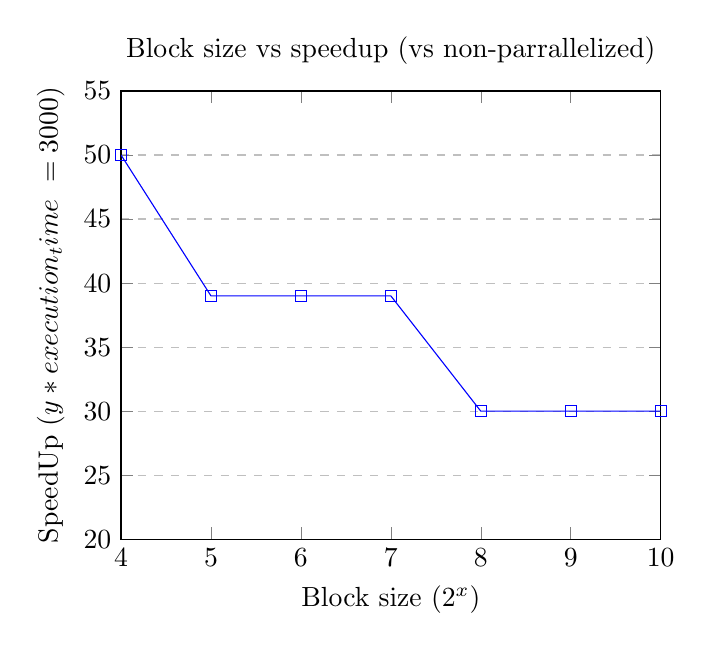
\begin{tikzpicture}
        \centering
        %%define axes
        \begin{axis}[
            title={Block size vs speedup (vs non-parrallelized)},
            xlabel={Block size ($2^x$)},
            ylabel={SpeedUp ($y*execution_time ~= 3000$)},
            xmin=4, xmax=10,
            ymin=20, ymax=55,
            xtick={4,5,6,7,8,9,10},
            ytick={20, 25, 30, 35, 40, 45, 50, 55},
            legend pos=north west,
            ymajorgrids=true,
            grid style=dashed,
        ]
        %% data filing
        \addplot[
            color=blue,
            mark=square,
            ]
            coordinates { %% Remind : axis X = 2^x
            (4, 50)(5,39)(6,39)(7,39)(8,30)(9,30)(10,30)
            };

        \end{axis}
    \end{tikzpicture}
    \newline
    We can see that we gain some times by using GPU, but the more you use an important number of blocks, the more you will lost time in parralelization computing. 
    \newLine 
    However, there is a difference between the initial image and the processed gray-scaled image : 
    
    \begin{verbatim}
        # ls -ll ../data/eiffel.jpg && ls -ll ./labwork3-gpu-out.jpg
        [...] 1865948 [...] ../data/eiffel.jpg
        [...] 1910376 [...] ./labwork3-gpu-out.jpg

    \end{verbatim}
    
\end{document}

